\documentclass[prl,twocolumn,superscriptaddress]{revtex4}
% \documentclass[twocolumn, a4j]{jarticle}
\usepackage[dvipdfmx]{graphicx,color}
\usepackage{amsmath,amssymb,braket,float,bm,color,comment,physics}
% \usepackage{mathabx}
\begin{document}

\title{Transport Phenomena of Granular Materials in a Highly Filled Rotating Cylindrical System}
% 高充填回転円筒系における粒体の輸送現象

\author{Shoichi Yoneta}
\affiliation{Dept. of Physics, Kyushu University}

\author{Shio Inagaki}
\affiliation{Dept. of Physics, Kyushu University}

\date{\today}

\begin{abstract}
同心二重円筒内に単種粒子を詰めて, 円筒の中心軸を水平にして回転させることで高充填単分散系における移流構造を調べた.本実験は白色粒子と色だけ異なる着色粒子を用いる.回転中の円筒の表面と回転後の断面の観察および,着色パルスの軌跡から速度の導出を行うことで,円筒内の移流を定量化した.実験から分かった移流構造の特徴を満たす軸方向速度分布モデルを提案する.非圧縮性物質の仮定と質量保存則から導かれる流量の保存を用いて, 円筒内全域における速度場を導出した.また,モデルの妥当性を評価するため,速度場が空間依存する移流方程式を立式し,着色粒子の存在比率を有限差分法によって求めた.最後に,実験によって得られた観測値とシミュレーションによって得られた数値解を比較して,モデルの定性的な評価を行った.
\end{abstract}
\maketitle

% \paragraph{I. INTRODUCTION:}
%%%%%%%%%%%%%%%%%%%%%%%%%%%%%%%%%%%%%%%%%%%%%%%%%%%%%%%%%%%%%%%%%%
%%%%%%%%%%%%%%%%%%%%%%%%%%%%%%%%%%%%%%%%%%%%%%%%%%%%%%%%%%%%%%%%%%
{\bf I. 導入} \\
食品,医薬品,化学の製造プロセスにおいて混合を行うことがある.粉体の混合への理解は重要.\\

粉粒体には通常の流体や固体には見られない興味深い特性がある.その一例として,二分散系における分離現象がある.高充填二分散系の例として,円筒容器内にいれ,回転させると分離現象が起こり,円筒の表面において中央から両端への移流が観察されている \cite{Inagaki10, Inagaki15}.また直方体容器を用いた実験 \cite{Rietz08:rectangularExpt, Rietz12:rectangularExpt} および,シミュレーション\cite{Awazu00:rectangularSimu}の研究も行われている.実験においては,複数の渦が発生することがわかっている.また,部分充填二分散系において内部構造を探る試みは, MRI \cite{Hill97:MRI},  陽電子放出粒子追跡(PEPT) \cite{Ding01:PEPT}, 凝固剤による固化 \cite{Santomaso04:solid}などのさまざまな手法が使用されてきた.ただしこれらの手法は, 高額な実験装置が必要であったり, 実験に手間のかかる.また,高充填系は構造的に内部を観察することが困難である.
% 卓上塩を使った実験で内部がみえたのは意外だった. ガラスビーズで試してみた(黒色粒子はアルミナ1粒子)が, 下から照明を当てても見えなかった. 光が散乱して半透明になったのが原因かも?

今回我々は, 二分散系のサイズ分離現象時に見られた移流が単分散系においても確認できるか調べるために, 高充填単分散系における内部の観察を行った. 二分散系の場合は,自発的にバンドが形成されるため,移流を定量化することは比較的容易である.しかし,単分散系においてはバンドが形成されないため,初期状態において円筒内の一部に着色粒子を配置した.円筒を回転させ,この着色パルスの時間発展を観察することで,円筒内の移流を定量化した.この手法によって,単分散高充填系において円筒の表面だけでなく,内部の軌跡を非侵襲かつ継続的に可視化することに成功した.\\
% 内部の移流の連続的な時間発展を可視化した先行研究はあるのか?
% 一部の粒子を着色することで, 移流を可視化する手法を用いた. 実験後は脱色することで, 再利用を可能にした. \\
%%%%%%%%%%%%%%%%%%%%%%%%%%%%%%%%%%%%%%%%%%%%%%%%%%%%%%%%%%%%%%%%%%
%%%%%%%%%%%%%%%%%%%%%%%%%%%%%%%%%%%%%%%%%%%%%%%%%%%%%%%%%%%%%%%%%%
\\
{\bf I\hspace{-.1em}I. 実験方法と解析方法} \\
	実験はアクリル製の透明な同心二重円筒に単種粒子を入れて行った.この円筒は外円と内円の間に粒子を詰めることが可能である.円筒の内円の半径$r_i$は20 $\rm{mm}$, 外円の半径$r_s$は40 $\rm{mm}$, 長さ$L$は345 $\rm{mm}$である.回転実験の後に分離して内部を観察できるようにするために,円筒は2つの半円筒に切断し,ボルトで固定した.色が白,粒径が280±70 $\rm{\mu m}$,密度が3.8 $\rm{g/cm^3}$の球状のアルミナビーズを使用した.そして,円筒内の流れが観察できるように,色の異なる粒子(白と赤)を使用した.赤色の粒子は,既製品である白のアルミナビーズ(アズワン AL9-0.3)をマジックインキで着色して作った.直立にした円筒に,白色粒子と着色粒子を交互に詰めて,充填率を95 $\%$にした.充填率は円筒に入れた粒子の体積を円筒の容積の64 $\%$(Random close packing \cite{Pouliquen97:RCP})で正規化した値として定義する.着色パルスの位置を測ることで,粒子の流れを観察することができます.この円筒をタイヤのついた平行な2本の軸上に水平においた.片方の軸をブラシなしモータ(Oriental Motors)で駆動することにより,円筒を一定の回転数(15 \rm{rpm})で回転させた.回転中は円筒の表面を一定時間毎に撮影した.画像をグレーに変換したため,着色粒子が黒く表示されている.これらの画像シーケンスから,時空間プロットを作成した.時空間プロットの横軸が軸方向空間, 縦軸が時間である.時空間プロットは各時間の円筒表面の軸方向ベクトルを垂直に結合することで作成した.この実験方法は稲垣氏\cite{Inagaki15}が用いた方法と本質的に同じである.\\

%%%%%%%%%%%%%%%%%%%%%%%%%%%%%%%%%%%%%%%%%%%%%%%%%%%%%%%%%%%%%%%%%%
%%%%%%%%%%%%%%%%%%%%%%%%%%%%%%%%%%%%%%%%%%%%%%%%%%%%%%%%%%%%%%%%%%

{\bf I\hspace{-.1em}I\hspace{-.1em}I. 実験結果と考察} \\
\begin{figure}[tb]
	\centering
	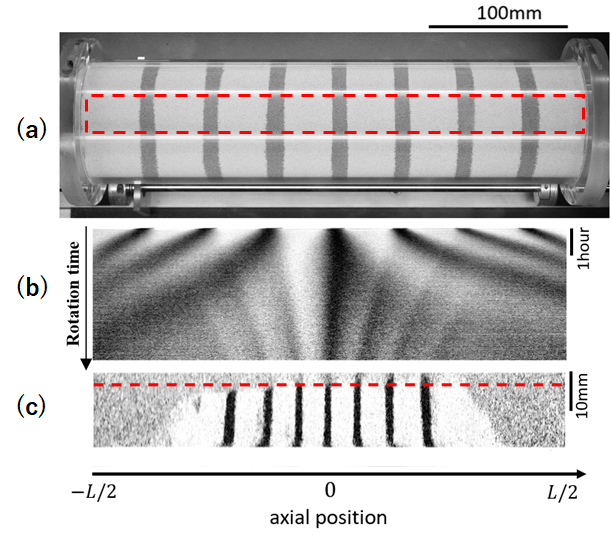
\includegraphics[width=0.5\textwidth]{figure/24_gray.png}
	\caption{実験1は充填率95%,回転時間が5時間である.(a-1) セットアップの画像.円筒を上から撮っている. (a-2) 時空間プロット. (a-3) 断面 見やすさのため断面のアスペクト比を変更している.}
	\label{fig:Expt.1}
\end{figure}

まず, 流れの全体像を観察するために, 初期状態において7本の着色パルスを等間隔に配置した(Fig. \ref{fig:Expt.1}(a))実験1を行った.時空間プロット(Fig. \ref{fig:Expt.1}(b))は円筒表面の時間経過を示している.時空間プロットから,着色パルスの初期位置から両端へ移動する7本の濃い軌跡が確認できる.このことから円筒の表面では中央から両端への流れが起きていることがわかる.また時空間プロットから,中央へ向かう薄い軌跡が確認できる.5時間の回転後に円筒を2つに分離し,内部を観察した.Fig. \ref{fig:Expt.1}(c)は二重円筒の断面のうちの1つである.図の上側が円筒の外円、下側が内円である.断面を観察すると,円筒内部が二つの領域があることがわかる.

内部中央付近は,着色パルスが平行な状態を維持したまま中央へ移動していることがわかる.
非混合領域の着色パルスの位置と時空間プロット上の薄い軌跡の最終位置が一対一対応していることがわかる.この結果が示唆することは,薄い軌跡は非混合領域から表面に湧き出す着色粒子の時間発展である,ということである.
%前回ここまで
また,両端の着色パルスの軌跡が端において漸近していないことから,側壁での速度がゼロでないことがわかる.

表層の厚みは,円筒中央付近の混合領域の厚みと同じ,かつ軸方向位置によらず一定と仮定した.断面上の層境界を破線で表す.層境界より上側を「表層」, 下側を「内層」と呼ぶことにする.なお,円筒の端付近において層境界と領域(混合と非混合)境界が一致しないのは,表層で混合された粒子が端付近で内部に沈み込みからである.

まとめると, 薄い軌跡からわかるように, 内層においては粒子は両端から中央へ移動する. 中央では粒子は表層へ湧き出している. 濃い軌跡からわかるように, 表層において粒子は中央から両端へ移動する. 両端においては, 粒子は内層に沈み込む. このように円筒の内部構造は,右半分に時計回り,左半分に反時計回りの2つの渦構造になっていると考えられる.データから得られた最も驚くべき結果は,非侵襲的に内層の着色パルスの位置がわかることである.\\

\begin{figure}[tb]
	\centering
	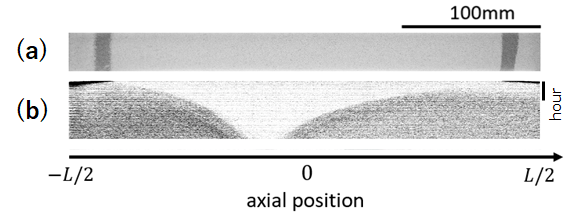
\includegraphics[width=0.5\textwidth]{figure/42_gray.png}
	\caption{実験2は充填率95%,回転時間が??時間である. (b-1) セットアップの直方領域の画像  (b-2) 時空間プロット.}
	\label{fig:Expt.2}
\end{figure}
次に内層の軸方向速度を定量化するために, 初期状態において円筒の両端付近に1本ずつ,計2本の着色パルスを配置した(Fig. \ref{fig:Expt.2}(a))のが実験2である.時空間プロットから端へ向かう濃い軌跡と中央へ向かう薄い軌跡が確認できる.薄い軌跡の内端が内層の軌跡と考えられる.内層の軌跡が〇時間後に合流していることから,移流構造の中心で速度がゼロでないことがわかる.\\

\begin{figure}[tb]
	\centering
	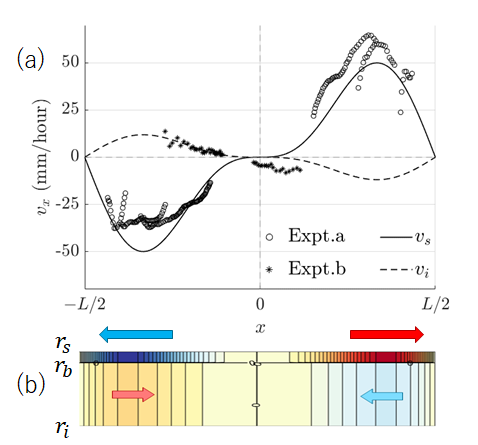
\includegraphics[width=0.5\textwidth]{figure/observed_and_model_vx.png}
	\caption{$v_x$の観測値とモデル.実験1から得られた表層軌跡の速度分布(o). 実験2から得られた内層軌跡の速度分布(*).}
	\label{fig:profile_model_vx}
\end{figure}
Fig. \ref{fig:Expt.1}(b)の濃い軌跡とFig. \ref{fig:Expt.2}(b)の薄い軌跡から速度を計算し,Fig. \ref{fig:profile_model_vx}(a)にプロットした.円筒の中心を原点とする軸方向位置を$x$,軸方向速度は$v_x$と定義する.\\
%%%%%%%%%%%%%%%%%%%%%%%%%%%%%%%%%%%%%%%%%%%%%%%%%%%%%%%%%%%%%%%%%%
%%%%%%%%%%%%%%%%%%%%%%%%%%%%%%%%%%%%%%%%%%%%%%%%%%%%%%%%%%%%%%%%%%

{\bf I\hspace{-.1em}V. モデリング} \\
\qquad{\bf 1. $x-v_x$分布モデルの提案} \\
実験から得られた速度分布の特徴を満たす,$x-v_x$分布の簡易モデルを提案する.$x=0$面における移流構造の左右対称性,各層内における$v_x$の動径方向非依存性,軸対称性,各層において速度場が滑らかであると仮定する.これらの条件を満たす$v_x$として, $v_x \propto f(a, b) \equiv \sin(2\pi \tilde{x})-a\sin(b\cdot 2\pi \tilde{x})$と定める.$\tilde{x}(\equiv x/L)$はドラム長で正規化した軸方向位置である.表層の軸方向速度を$v_s$,表層の軸方向最高速度を$v_{smax}$とする.$v_s \equiv N_sf$の最大値が$v_{smax}$になるようにフィッティングパラメータ$N_s$を定める.実験1の速度分布に近くなるように,モデルは$v_{smax}=50 (\rm{mm/hour})$とした(Fig. \ref{fig:profile_model_vx}(a)).両端や移流構造の中心で速度がゼロでないことから,$v_s=f(0.4, 1.5)$とした.\\
%%%%%%%%%%%%%%%%%%%%%%%%%%%%%%%%%%%%%%%%%%%%%%%%%%%%%%%%%%%%%%%%%%
\\
\qquad{\bf 3. 2次元定常速度場の導出} \\
2次元定常速度場を導出する.粒子は非圧縮性物質であると仮定することで, 全粒子系における質量保存則から, 非圧縮性流れが導ける. ガウスの発散定理より, 任意の体積領域の表面$S$で総流量がゼロ$\qty(\iint\nolimits_S\vb*{n}\vdot\vb*{v}dS = 0)$となる.$\vb*{v}$は速度である.つまり, 表面$S$上を通過する粒子の流入量と流出量が等しくなる.流量保存から,表層と内層の軸方向速度の関係, 内層における軸方向速度と動径方向速度の関係を導出する.

まず,表層の軸方向速度から内層の軸方向速度を導出する.内層の軸方向速度を$v_i$,円筒中心軸から層境界までの距離を$r_b$と定義する.簡単のため,円筒内に粒子が十分に満たされていることを仮定する.また実験1より,各層内における$v_x$の動径方向非依存性を仮定する.ここで二重円筒領域$V_1$の表面における流量保存を考える. 領域$V_1$の動径方向の範囲は$[r_i, r_s]$, 軸方向の範囲は$[x', L/2]$である.$x=x'$面(以降,$S_{x'}$面と呼ぶ)の各層内における$v_x$は一様である.$S_{x'}$面における,表層と内層の面積を$S_s, S_i$とする.領域$V_1$の表面積のうち,粒子の流入出があるのは$S_{x'}$面だけである.$S_{x'}$面における流量保存$(S_iv_i+S_sv_s = 0)$より,$v_i = -N_sS_s/S_i(\sin(2\pi \tilde{x})-0.4\sin(1.5\cdot 2\pi \tilde{x}))$.よって,$v_s$から$v_i$を導出できた.Fig. \ref{fig:profile_model_vx}(b)は断面における$v_x$の定常速度場モデルである.\\

次に, 内層内において軸方向速度から動径方向速度を導出する. 円筒中心軸からの動径方向距離を$r$,動径方向速度は$v_r$と定義する.
回転軸対称と内層における$v_x$の$r$非依存性の仮定より, 円筒座標系における非圧縮性流れの式から \\
\begin{eqnarray*}
v_r = -\dfrac{1}{2}\dv{v_i}{x}r+\dfrac{C(x)}{r}
\end{eqnarray*}
となることがわかる. $C(x)$は積分定数.内層内について考えているので, $v_x$を$v_i$としている. ここで内層内の二重円筒領域$V_2$の表面における流量保存を考える(Fig. \ref{fig:vx_and_vr}). 領域$V_2$の動径方向の範囲は$[r_i, r]$, 軸方向の範囲は$[x, x+\Delta x]$である. 領域の$V_2$は内層内なので, $r$は内層内($r_i < r\leqslant r_b$)の任意の値をとる. Fig. \ref{fig:vx_and_vr} の二重円筒領域$V_2$において, 軸方向に垂直な2つの面(赤い面)と, 動径方向に垂直な外側の側面(青い面)からの流出量が等しくなるという流量保存 \\
\begin{eqnarray*}
\pi\qty(r^2-{r_i}^2)\qty(v_i(x+\Delta x)-v_i(x)) + \displaystyle\int_{x}^{x+\Delta x}dx\int_{0}^{2\pi}d\theta\hspace{2pt}v_rr \\
= 0 \\
\end{eqnarray*}
から,$v_r$が導ける \cite{supplement}.
\begin{eqnarray} \label{eq:vx_vr}
v_r(r,x) = -\dfrac{1}{2}\dv{v_i(x)}{x}\qty(r-\dfrac{{r_i}^2}{r})
\end{eqnarray}
なお流量の保存において, 二重円筒領域$V_2$の内側の側面を考慮しなかったのは, 粒子の流入出がないからである. よって, 先ほど導出した$v_i$から内層の$v_r$が導出できる.Fig. \ref{fig:model_vr}(a)は層境界上の$v_r$の速度分布である.Fig. \ref{fig:model_vr}(b)は断面における$v_r$の定常速度場モデルである.\\
\\*

\begin{figure}[tb]
	\centering
	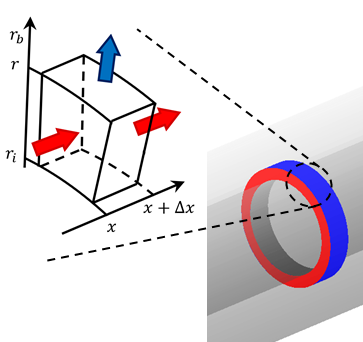
\includegraphics[width=0.5\textwidth]{figure/vx_vr_inner4.png}
	\caption{内層における軸方向速度と動径方向速度の関係の導出}
	\label{fig:vx_and_vr}
\end{figure}
\begin{figure}[tb]
	% \vskip10mm
	\centering
	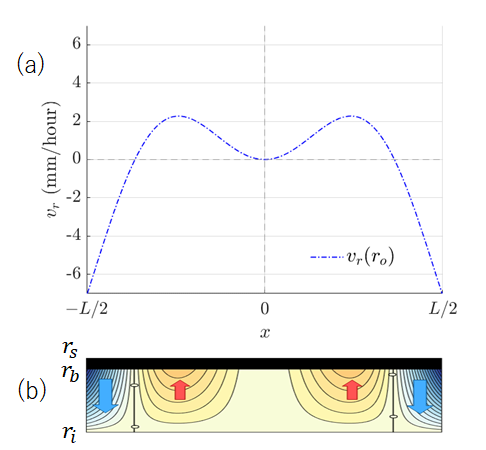
\includegraphics[width=0.5\textwidth]{figure/model_vr.png}
	\caption{$v_r$のモデル.表層はピストン流なので, $r$方向の拡散は無限大である. そのため表層の$v_r$は定義不可である.}
	\label{fig:model_vr}
\end{figure}

%%%%%%%%%%%%%%%%%%%%%%%%%%%%%%%%%%%%%%%%%%%%%%%%%%%%%%%%%%%%%%%%%%
{\bf V. シミュレーション} \\
\qquad{\bf 1. 支配方程式} \\
モデルの妥当性を評価するために,数値シミュレーションを行う.シミュレーションの支配方程式は移流方程式とする.支配方程式を導出する.全粒子系の密度, フラックス, 速度を$\rho, \vb*{j}, \vb*{v}$, 着色粒子系の場合は, $\rho_A, \vb*{j_A}, \vb*{v_A}$と定義する.本研究の実験は白色粒子と着色粒子の二成分系のパッシブスカラー輸送を想定している. パッシブスカラー輸送とは, 着色粒子の存在比率が速度場に影響を与えず, 速度場に従う輸送現象のことである.パッシブスカラー輸送より, $\vb*{v} = \vb*{v_A}$となる. フラックスは拡散を考慮せず移流のみと仮定する$(\vb*{j} = \rho\vb*{v},\hspace{5pt}\vb*{j_A} = \rho_A\vb*{v_A})$.パッシブスカラー輸送, 非圧縮性, 回転軸対称の仮定と, 着色粒子系の質量保存則$\qty(\partial\rho_A/\partial t+\div{\vb*{j_A}}=0)$から円筒座標系における移流方程式 
\begin{equation} \label{eq:2Dae}
\pdv{\phi_A}{t}+v_x\pdv{\phi_A}{x}+v_r\pdv{\phi_A}{r} = 0
\end{equation}
が導ける \cite{supplement}.なお,$v_x, v_r$は全粒子系における速度,存在比率$\phi_A(\equiv\rho_A/\rho)$は正規化した$\rho_A$である.これより,着色粒子系における移流方程式を解くためには,全粒子系における定常速度場モデル(Fig. \ref{fig:profile_model_vx},Fig. \ref{fig:model_vr})を使用すればよいことがわかる.\\
%%%%%%%%%%%%%%%%%%%%%%%%%%%%%%%%%%%%%%%%%%%%%%%%%%%%%%%%%%%%%%%%%%
%%%%%%%%%%%%%%%%%%%%%%%%%%%%%%%%%%%%%%%%%%%%%%%%%%%%%%%%%%%%%%%%%%
\\
\qquad{\bf 2. シミュレーション手法} \\
軸対称より,周方向$\theta$を除いた,断面(軸方向と動径方向)の2次元シミュレーションを行う.有限差分法を用いて$\phi_A$を計算する.偏微分方程式の非定常項は前進オイラー法,移流項は1次精度風上差分の陽解法によって,離散化した.計算点にはスタガード格子を, 境界条件はノイマン条件を選択した. 数値計算における数値の発散を回避するため, CFL条件($\Delta t\qty(|v_x|/\Delta x+|v_r|/\Delta r)\leqslant1$) \cite{supplement, LeVeque07:FDM}を満たすように刻み幅を設定した.$\Delta x,\hspace{5pt}\Delta r,\hspace{5pt}\Delta t$ はそれぞれ軸方向, 動径方向, 時間の刻み幅であり, $\Delta x = \Delta r = 0.15 \rm{(mm/cell)}, \hspace{5pt}\Delta t = 4.5 (\rm{sec/step})$とした.表層の流れがピストン流なので$v_r$が定義できないが, シミュレーションを行うには表層の$v_r$の値を決めなければいけない.そのため, 内層の$v_x$と$v_r$の関係と同様に, 表面における流量の保存から表層の$v_r$を導出し, これをシミュレーション上の便宜的な表層の$v_r$とした.そして表層における流れがピストン流であることを反映させるため,各ステップごとに有限差分法による計算の後に,表層内の$\phi_A$を動径方向に均一になるように平均化した.この処理は$\phi_A$の総量保存を破らない.\\
%%%%%%%%%%%%%%%%%%%%%%%%%%%%%%%%%%%%%%%%%%%%%%%%%%%%%%%%%%%%%%%%%%
%%%%%%%%%%%%%%%%%%%%%%%%%%%%%%%%%%%%%%%%%%%%%%%%%%%%%%%%%%%%%%%%%%
\\
\qquad{\bf 3. シミュレーション結果} \\
\begin{comment}
\begin{figure}[t]
	\begin{minipage}[t]{0.95\linewidth}
		\centering
		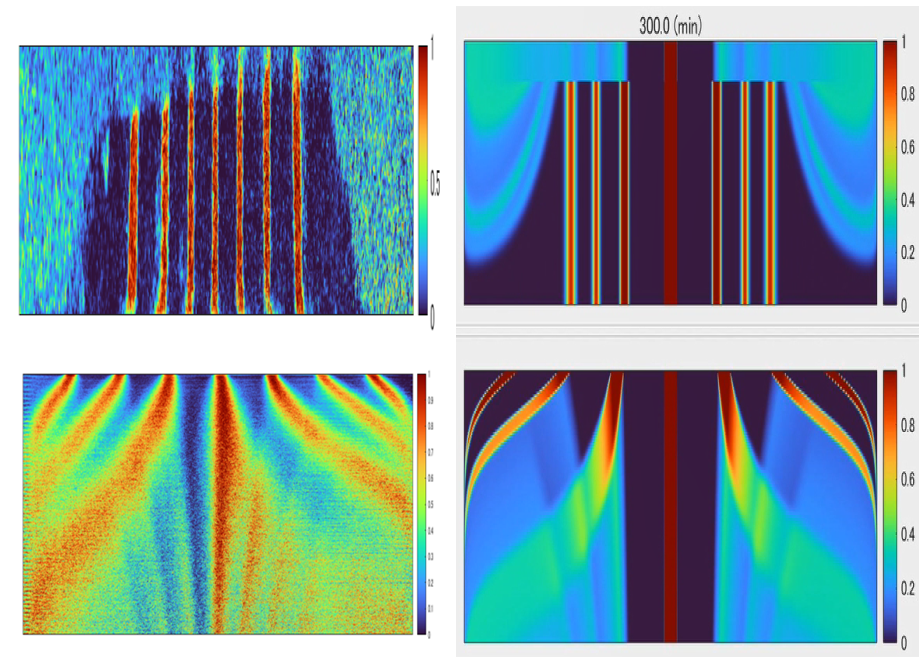
\includegraphics[width=\textwidth]{figure/24_exp_and_simu.png}
	\end{minipage}
	\begin{minipage}[t]{0.95\linewidth}
		\centering
		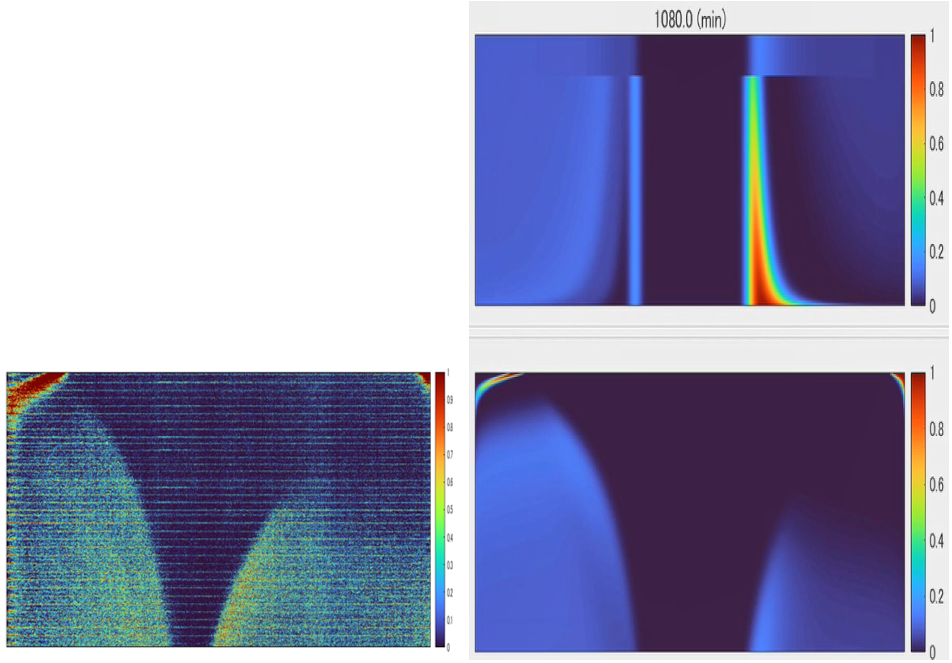
\includegraphics[width=\textwidth]{figure/38_exp_and_simu.png}
	\end{minipage}
	\caption{実験とモデルのシミュレーションの比較 (a)全体像 (b)両端}
	\label{fig:simu}
\end{figure}
\end{comment}

\begin{figure*}[t]
 \begin{center}
  \includegraphics[width=\textwidth]{figure/24_43_heatmap2.bmp}
  \caption{実験とモデルのシミュレーションの比較 (a)全体像 (b)両端}
  \label{}
 \end{center}
\end{figure*}
シミュレーション結果と実験を比較することでモデルを定性的に評価した.Fig. \ref{fig:simu}(a) は実験1の実験結果とモデルのシミュレーションである.まず断面の比較をする.表層の端付近に到達した白色粒子と着色粒子の混合粒子が, 内層の端の上部から中央に向かって徐々に広がっていく様子が実験で観察されたが, モデルのシミュレーションにおいても同様の特徴が現れている. なおモデルの支配方程式は移流方程式であるため, 表層の中央で拡散が見られない点が実験の特徴と異なる. 次に時空間プロットの比較をする.シミュレーションの時空間プロットは,実験と同様に各時間の円筒表面(断面のシミュレーションの最上行)の軸方向ベクトルを下に結合することで作成した.モデルは移流構造が左右対称であるが, 実験では移流構造の中心が円筒の中心より左にある点に注意する. 中央と両端における着色パルスの軌跡の特徴は, 実験とモデルでおおむね一致していることがわかる. なおモデルでは端で速度が0に漸近しているがこれは実験の特徴と異なる.  Fig. \ref{fig:simu}(b) は実験2の実験結果とモデルのシミュレーションである.初期段階では内層の軌跡が表れず, 途中から表れているという実験の特徴がシミュレーションにおいても表れている.シミュレーションの結果に対して, $\phi_A$の総量保存の検証を行ったところ,全て相対誤差/hourが1%未満となった. 他にもモデルを正確に解けているかの検証として, モデルの速度分布とシミュレーション結果から取得した速度分布の比較やモデルの流れ関数\cite{Batchelor00:fluid}から求まる流跡線の解析解とシミュレーションのトレーサ粒子の軌跡を比較した.その結果,モデルを十分精度よく解けていることが確認できた \cite{supplement}.\\
%%%%%%%%%%%%%%%%%%%%%%%%%%%%%%%%%%%%%%%%%%%%%%%%%%%%%%%%%%%%%%%%%%
%%%%%%%%%%%%%%%%%%%%%%%%%%%%%%%%%%%%%%%%%%%%%%%%%%%%%%%%%%%%%%%%%%
\\
{\bf V\hspace{-.1em}I. 結論} \\
要約すると,実験から高充填二分散系の回転二重円筒内の粒子は渦型に移流することが確認できた.円筒中央において粒子が湧き出すことから,非侵襲的な表面観察だけで内層の速度分布を定量化することが可能になった.保存則に従い, かつ移流構造の特徴を捉えたモデルの提案を行った.二分散系において,サイズ分離により形成されたバンドが中央から両端に移流する現象が報告されているが,本研究により,二分散系由来のサイズ分離現象がなくとも,移流が起こることがわかった.
円筒を回転させると渦構造が形成される要因については,遠心力と壁面摩擦によるものであるという仮説を提案する.$r$が一定のとき,任意の軸方向位置において,遠心力は均一に働いているが,壁面は摩擦により相対的に中央よりも遠心力の影響が弱くなる.その結果,表層において中央で密に,両端で疎になる偏りが発生する.その偏りを緩和するために,表層においては中央から両端に粒子が流れると考える.同様の議論により,内層においては両端から中央に粒子が流れる.

今後の課題としては,3つのことを検討している.1つ目は,定量的なモデルの妥当性評価である.定性的には,モデルのシミュレーションは実験の特徴をよくとらえてるが定量的な評価はまだできていない.定量的にモデルの妥当性を評価するには,多くの実験データを必要とする.2つ目は,拡散を考慮したモデルの提案である.本モデルは移流方程式を支配方程式としており,拡散を考慮しないモデルとなっている.移流拡散方程式を支配方程式とする拡散を考慮したモデルを設計することにより,実験結果のより詳細な再現が可能になるかもしれない.シミュレーションにおいて拡散の発生が確認できるのは,速度場の空間依存性により,移流方程式が非線形になっているからである.例えば,Fig. \ref{fig:simu}(a-4)の左から3, 5番目のパルス拡散により幅が広がっている.3つ目は円筒の回転速度や充填率などのパラメータと速度場の関係の解明である.\\

\begin{thebibliography}{}
\bibitem{Inagaki10}
S. Inagaki and K.Yoshikawa, {\it{Phys. Rev. Lett.}} {\bf 105}, 118001 (2010).
\bibitem{Inagaki15}
S. Inagaki, H. Ebata and K.Yoshikawa, {\it{Phys. Rev. E}} {\bf 91}, 010201(R) (2015).
\bibitem{Rietz08:rectangularExpt}
F. Rietz and R. Stannarius, {\it{Phys. Rev. Lett.}} {\bf 100}, 078002 (2008).
\bibitem{Rietz12:rectangularExpt}
F. Rietz and R. Stannarius, {\it{Phys. Rev. Lett.}} {\bf 108}, 118001 (2012).
\bibitem{Awazu00:rectangularSimu}
A. Awazu, {\it{Phys. Rev. Lett.}} {\bf 84}, 4585 (2000).
\bibitem{Hill97:MRI}
K. M. Hill, A. Caprihan, and J. Kakalios, {\it{Phys. Rev. Lett.}} {\bf 78}, 50 (1997).
\bibitem{Ding01:PEPT}
Y. L. Ding, J. P. K. Seville, R. Forster and D. J. Parker, {\it{Chem. Eng. Sci.}} {\bf 56}, 1769-1780 (2001).
\bibitem{Santomaso04:solid}
A. Santomaso, M. Olivi and P. Canu, {\it{Chem. Eng. Sci.}} {\bf 59}, 3269-3280 (2004).
\bibitem{Pouliquen97:RCP}
O. Pouliquen, M. Nicolas, and P. D. Weidman, {\it{Phys. Rev. Lett.}} {\bf 79}, 3640 (1997).
\bibitem{supplement}
See Supplemental Material at .
\bibitem{LeVeque07:FDM}
R. J. LeVeque, {\it{Finite Difference Methods for Ordinary and Partial Differential Equations}} (University of Washington, Washington, 2007).
\bibitem{Batchelor00:fluid}
G. K. Batchelor, {\it{AN INTRODUCTION TO FLUID DYNAMICS}} (Cambridge University Press, Washington, 2000).
\end{thebibliography}

\end{document}